\section{Auswertung}
\label{sec:Auswertung}

\subsection{Darstellung der Moden}
Die Reflektorspannungen $U$, die Spannungsamplituden $A$, sowie Frequnenzen $f$ für drei verschiedene Moden sind in Tabelle 1 dargestellt.
Die Stromstärke beträgt dabei $I = 25$mA.



\begin{table}[H]
  \centering
  \caption{Reflektorspannungen, die Spannungsamplituden und die Frequnenzen der drei Moden}
  \label{tab:Parameter}
  \begin{tabular}{c c c c}
    \toprule
    Mode & $U/$V & $A/$mV& $f/$s\\
    \midrule
    1. & 83  &   119.9& 8999 \\
       & 95  & &       \\
       & 105 & &       \\
    2. & 135 &   152.4 & 8994 \\
       & 150 & & \\
       & 165 & & \\
    3. & 215 &   138.7 & 8988 \\
       & 230 & & \\
       & 245 & & \\
    \bottomrule
  \end{tabular}
\end{table}

\begin{figure}
  \centering
  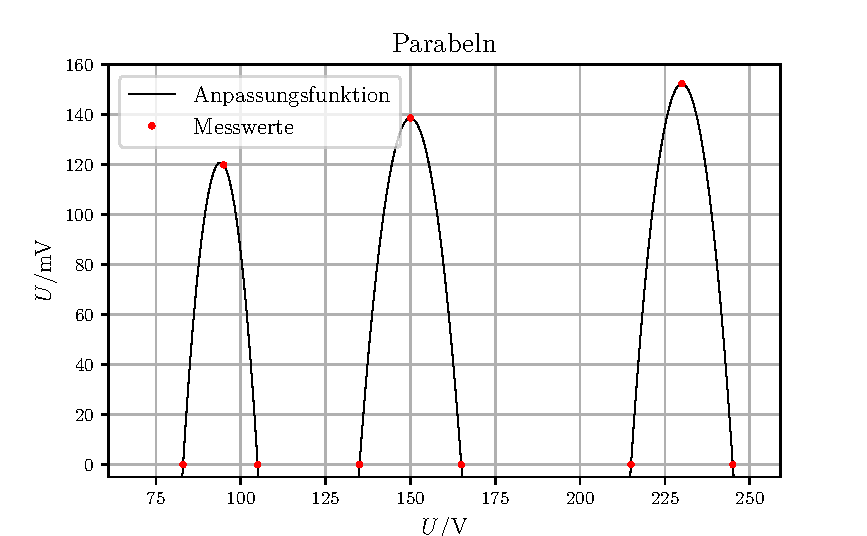
\includegraphics{plot1.pdf}
  \caption{Anpassungsfunktionen für die Messwerte der drei Moden}
  \label{fig:plot}
\end{figure}
